\documentclass[10pt]{extarticle}

\usepackage[margin=0.2in]{geometry}

\usepackage{graphicx}
\usepackage{libertine}
\usepackage{libertinust1math}
\usepackage[T1]{fontenc}

\usepackage{amsmath, amssymb}

\usepackage{enumitem}
\usepackage{multicol}
\usepackage{multirow}

\usepackage{bytefield}

\usepackage{titlesec}

\usepackage{tikz}
\usetikzlibrary{shapes.geometric, arrows, positioning}

\titlespacing\subsection{0pt}{0pt}{0pt}
\titlespacing\subsubsection{0pt}{-1em}{0pt}
\titlespacing\paragraph{0pt}{0pt}{3pt}
\titlespacing\subparagraph{0pt}{0pt}{2pt}

\setdescription{itemsep=-5pt}
\setenumerate{itemsep=0pt}
\setitemize{itemsep=-5pt}

\setlength{\jot}{0em}

\begin{document}
\begin{multicols}{2}
  \begin{description}
    \item[Metcalfe's Law] The value of a network grows \(O(n^2)\), where \(n\) is the number of nodes in a network.
    \item[Baud Rate] The number of signal changes per second.
    \item[Bandwidth] The bits per second that can be transmitted. \\
          \hspace*{-2em}
          \(\text{Data Rate} = \text{Baud Rate (symbols/second)} \times
          \log_2 \left( \text{\# of distinct symbols} \right) \)
    \item[Simple and Inexpensive] Ethernet is simple and inexpensive to implement.
    \item[Shared Medium] All devices on a network share the same medium. (Defunct)
    \item[Carrier Sense Multiple Access w/ Collision Detection (CSMA/CD)]
          Devices listen before transmitting. If collision detected, devices
          wait a random amount of time before retransmitting. (Defunct)
    \item[MAC] Consists of 48 bits, with the first 24 bits being the Organizationally Unique
          Identifier (OUI).
          \begin{description}
            \item[Broadcast Address] \texttt{FF:FF:FF:FF:FF:FF}
            \item[Multicast Address] First bit 1. \\ (e.g. \texttt{01:00:5E:00:00:01})
            \item[Local Address] Second-least sig. bit 1. \\ (e.g. \texttt{02:00:00:00:00:01})
          \end{description}
  \end{description}

  \hspace{0.5em}
  \small
  \begin{tabular}{|c|c|p{0em}|c|c|c|c|l|}
    \cline{0-1}
    \cline{4-8}
    Application                & HTTP, FTP, \dots             &     & \multicolumn{4}{|c|}{all 0s}
                               & This host                                                                                                \\
    \cline{0-1}
    \cline{4-8}
    Transport                  & TCP, UDP                     &     & \multicolumn{2}{|c|}{all 0s} &
    \multicolumn{2}{|c|}{host} & Host on network                                                                                          \\
    \cline{0-1}
    \cline{4-8}
    Internet                   & Datagrams                    &     & \multicolumn{4}{|c|}{all 1s}
                               & Local broadcast                                                                                          \\
    \cline{0-1}
    \cline{4-8}Link            & MAC, Frames                  &     &
    \multicolumn{2}{|c|}{net}  & \multicolumn{2}{|c|}{all 1s} & Net
    broadcast                                                                                                                             \\
    \cline{0-1}
    \cline{4-8}Physical        & Ethernet, WiFi               &     & 127                          & \multicolumn{3}{|c|}{any} & Loopback \\
    \cline{0-1}
    \cline{4-8}
  \end{tabular}
  \normalsize

\end{multicols}

\small
\begin{tabular}{|c|l|c|l|}
  \hline
  \textbf{Device}                   & \textbf{Function}                                & \textbf{Layer}                   & \textbf{Key Characteristics} \\
  \hline
  \text{Repeater}                   & \text{Amplifies or regenerates signals to extend
  transmission distance}            & Physical
                                    & \text{Signal Amplification}
  \\
  \hline
  \text{Hub}                        & \text{Connects devices in a network,
  broadcasting data to all devices} & \multirow{3}{*}{Data Link}
                                    & \text{Simple, No intelligience / learning}                                                                         \\
  % \hline
  \cline{0-1}
  \cline{4-4}
  \text{Bridge}                     & \text{Filters traffic between two
  networks, forwards based on MAC}  &                                                  & \text{Reduces collision domains}
  \\
  \cline{0-1}
  \cline{4-4}
  \text{Switch}                     & \text{Smart HUB that forwards based on
  MAC}                              &                                                  & \text{Learns MAC addresses}
  \\
  \hline
\end{tabular}


\hspace{-3em}
% \begin{tabular}{|l|l|l|l|}
%   \hline
%   \textbf{Feature}       & \textbf{Thicknet}                                &
%   \textbf{Thinnet}       & \textbf{Twisted-Pair Ethernet
%   }                                                                                                                                              \\ \hline
%   \textbf{Alias}         & 10BASE5                                          & 10BASE2                          & 10BASE-T \dots                  \\ \hline
%   \textbf{Medium}        & Coaxial cable, 0.5-inch diameter                 & Coaxial cable, 0.2-inch diameter & Twisted pairs of copper wires   \\ \hline
%   \textbf{Max Length}    & 500 meters                                       & 185 meters                       & 100 meters (typical Cat5e/Cat6) \\ \hline
%   \textbf{Bandwidth}     & \multicolumn{2}{|c|}{10 Mbps}
%                          & 10 Mbps (higher for later versions)
%   \\ \hline
%   \textbf{Installation}  & Rigid and bulky, hard to install/manage          & Flexible, easier to install      & Easy to install and manage      \\ \hline
%   \textbf{Connector}     & N-type connectors                                & BNC connectors                   & RJ45 connectors                 \\ \hline
%   \textbf{Cost}          & Expensive                                        & Moderate                         & Low                             \\ \hline
%   \textbf{Amplification} & \multicolumn{2}{|c|}{Requires repeaters for long
%   distances}             & Hubs / switches for amplification
%   \\ \hline
%   \textbf{Flexibility}   & Low; bulky and inflexible                        & Moderate                         & High; widely used and adaptable \\ \hline
%   \textbf{Interference}  & Low (due to coaxial shielding)                   & Moderate                         & High without shielding          \\ \hline
% \end{tabular}
\normalsize

\vspace*{-1em}
\begin{multicols}{2}
  \begin{description}
    \item[DHCP] Dynamic IP assignment, uses UDP (server 67, client 68).
    \item[Mail Submission Agent (MSA)] Submits mail to the Mail Transfer Agent (MTA).
    \item[Mail Transfer Agent (MTA)] Transfers mail between servers.
    \item[Mail Delivery Agent (MDA)] Delivers mail to the recipient's mailbox.
    \item[Mail Retrieval Agent (MRA)] Retrieves mail from the mailbox.
    \item[Simple Mail Transfer Protocol (SMTP)] Used by the MSA and MTA.
    \item[Internet Message Access Protocol (IMAP)] Used by the MRA, allows for
          marking email as read.
    \item[Post Office Protocol 3 (POP3)] Used by the MRA, worse IMAP.
  \end{description}


  \begin{multicols}{2}
    \subsubsection*{Classful Addressing}
    \small
    \begin{tabular}{c|c|l}
      Class A & \texttt{0XXXXXXX} & /8  \\
      Class B & \texttt{10XXXXXX} & /16 \\
      Class C & \texttt{110XXXXX} & /24 \\
      Class D & \texttt{1110XXXX} & /31 \\
      Class E & \texttt{1111XXXX} & /32 \\
    \end{tabular}
    \begin{description}
      \item[`This' network'] host bits 0.
      \item[Broadcast] host bits 1.
    \end{description}
    \normalsize
    \columnbreak
    \subsubsection*{TCP}
    \hspace*{-3em}
    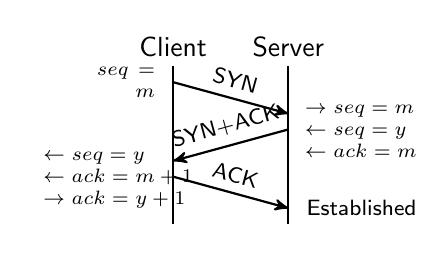
\begin{tikzpicture}[font=\sffamily\footnotesize,>=stealth',thick,
        header/.style={text width=1cm, align=center, font=\sffamily},
        commentl/.style={text width=1.0cm, align=right, font=\scriptsize},
        commentr/.style={commentl, align=left},]
      \node[header] (init) {Client};
      \node[header,right=0.2cm of init] (recv) {Server};

      \draw[->] ([yshift=-.2cm]init.south) coordinate (syn1a) --
      ([yshift=-.4cm]syn1a-|recv) coordinate (syn1b) node[pos=.5, above,
          sloped] {SYN};
      \draw[->] ([yshift=-.2cm]syn1b) coordinate (ack1a) --
      ([yshift=-.4cm]ack1a-|init) coordinate (ack1b) node[pos=.5, above, sloped]
        {SYN+ACK};
      \draw[->] ([yshift=-.2cm]ack1b) coordinate (ack2a) --
      ([yshift=-.4cm]ack2a-|recv) coordinate (ack2b) node[pos=.5, above, sloped] {ACK};

      \node[commentl, left=1mm of syn1a] {\(seq = m\)};
      \node[commentr, right=0mm of syn1b] {\begin{align*}
           & \rightarrow seq = m  \\
           & \leftarrow seq = y   \\
           & \leftarrow ack = m+1
        \end{align*}};
      \node[commentl, left=6mm of ack1b] {\begin{align*}
           & \leftarrow seq = y    \\
           & \leftarrow ack = m+1  \\
           & \rightarrow ack = y+1
        \end{align*}};

      \node[commentr, right=1mm of ack2b, font=\sffamily\footnotesize] {Established};

      \draw[thick, shorten >=-0.2cm] (init) -- (init|-ack2b);
      \draw[thick, shorten >=-0.2cm] (recv) -- (recv|-ack2b);
    \end{tikzpicture}
  \end{multicols}
\end{multicols}


\begin{multicols}{2}
  \vspace*{-3em}
  \begin{multicols}{2}
    \noindent
    \footnotesize
    \begin{bytefield}[bitwidth=4pt]{32}
      \bitheader{0, 16, 31} \\
      \bitbox{16}{SOURCE PORT} & \bitbox{16}{DESTINATION PORT} \\
      \bitbox{16}{LENGTH} & \bitbox{16}{CHECKSUM / 0} \\
      \wordbox{1}{DATA \dots} \\
    \end{bytefield}
    \begin{bytefield}[bitwidth=4pt]{32}
      \bitheader{0, 8, 16, 31} \\
      \wordbox{1}{SOURCE IP} \\
      \wordbox{1}{DESTINATION IP} \\
      \bitbox{8}{Zero} & \bitbox{8}{PROTO} & \bitbox{16}{UDP/TCP LENGTH} \\
    \end{bytefield} \\
    \hspace*{-2em}
    \scriptsize
    \begin{bytefield}[bitwidth=5pt]{32}
      \bitheader{0, 4, 10, 16, 24, 31} \\
      \bitbox{16}{SOURCE PORT} & \bitbox{16}{DESTINATION PORT} \\
      \bitbox{32}{SEQUENCE NUMBER} \\
      \bitbox{32}{ACKNOWLEDGEMENT NUMBER} \\
      \bitbox{4}{HLEN} & \bitbox{6}{RESV} & \bitbox{6}{FLAGS} &
      \bitbox{16}{WINDOW} \\
      \bitbox{16}{CHECKSUM} & \bitbox{16}{URGENT POINTER} \\
      \bitbox{24}{OPTIONS (IF ANY)} & \bitbox{8}{PADDING} \\
      \wordbox{1}{DATA \dots} \\
    \end{bytefield}
    \normalsize
  \end{multicols}
  \vspace*{-2.5em}

  \begin{multicols*}{2}
    \begin{description}
      \item[socket] Creates a socket
      \item[bind] Assigns an address to a socket
      \item[listen] Marks a socket as passive
      \item[accept] Accepts a connection request
      \item[connect] Initiates a connection
      \item[send] Sends data
      \item[recv] Receives data
      \item[close] Closes the socket
    \end{description}

    \paragraph*{Flow Control}
    \small
    \subparagraph*{Silly Window Syndrome} Data sent in inefficiently small chunks
    (high overhead). Either delay ACK and ad 0 window size (Clark's), or buffer data (Nagle's).
  \end{multicols*}

  \vspace*{-0.5em}
  Valid ports are \([1, 65535]\), with \([1, 1023]\) being privileged.

  \vspace*{-2em}

  \begin{align*}
    RTT                           & = \alpha \cdot RTT + (1 - \alpha) \cdot RTT_{\text{sample}} \\
    Timeout                       & = \beta \cdot RTT                                           \\
    \text{Upon Timeout} : Timeout & = \gamma \cdot \text{Timeout}
  \end{align*}


  \paragraph*{Congestion Control}
  \subparagraph*{Slow Start} \emph{Exponentially} increase window, till
  congestion window size.
  \subparagraph*{Congestion Avoidance} \emph{Linear} increase in window size.
  \subparagraph*{Karn's Algorithm} Multiply timeout by \(\gamma\) upon timeout.

  \paragraph*{RED}

  \columnbreak

  \vspace*{-5em}

  \begin{multicols}{2}
    \subsection*{TCP}
    \begin{itemize}
      \item Connection-oriented
      \item Stream-based
      \item Reliable
      \item High Overhead
    \end{itemize}

    \subsubsection*{Server}
    \begin{itemize}
      \item \texttt{socket}
      \item \texttt{bind}
      \item \texttt{listen}
      \item \texttt{accept}
      \item \texttt{send} / \texttt{recv}
      \item \texttt{close}
    \end{itemize}

    \subsubsection*{Client}
    \begin{itemize}
      \item \texttt{socket}
      \item \texttt{connect}
      \item \texttt{send} / \texttt{recv}
      \item \texttt{close}
    \end{itemize}

    \columnbreak

    \subsection*{UDP}
    \begin{itemize}
      \item Connectionless
      \item Message-based
      \item Unreliable
      \item Low Overhead
    \end{itemize}

    \subsubsection*{Server}
    \begin{itemize}
      \item \texttt{socket}
      \item \texttt{bind}
      \item \texttt{recvfrom}
      \item \texttt{sendto}
      \item \texttt{close}
    \end{itemize}

    \subsubsection*{Client}
    \begin{itemize}
      \item \texttt{socket}
      \item \texttt{sendto}
      \item \texttt{recvfrom}
      \item \texttt{close}
    \end{itemize}

  \end{multicols}

  % \vspace*{-3em}

  \scriptsize
  \begin{bytefield}{32}
    \bitheader{0, 8, 16, 31} \\
    \bitbox{4}{VERS} & \bitbox{4}{HLEN} & \bitbox{8}{SERVICE TYPE} &
    \bitbox{16}{TOTAL LENGTH} \\
    \bitbox{16}{IDENTIFICATION} & \bitbox{3}{FLAGS} & \bitbox{13}{FRAGMENT OFFSET}
    \\
    \bitbox{8}{TTL} & \bitbox{8}{PROTOCOL} & \bitbox{16}{HEADER CHECKSUM} \\
    \wordbox{1}{SOURCE IP} \\
    \wordbox{1}{DESTINATION IP} \\
    \bitbox{24}{IP OPTIONS (IF ANY)} & \bitbox{8}{PADDING} \\
    \wordbox{1}{DATA \dots} \\
  \end{bytefield} \\
  \begin{bytefield}{32}
    \bitbox[]{8}{Preamble} & \bitbox[]{6}{Destination Address} &
    \bitbox[]{6}{Source Address} & \bitbox[]{2}{Frame Type} & \bitbox[]{12}{Frame
      Data} & \bitbox[]{4}{CRC} \\
    \bitbox{8}{8 octets} & \bitbox{6}{6 octets} & \bitbox{6}{6 octets} &
    \bitbox{2}{2} & \bitbox{12}{46 - 1500 octets} & \bitbox{4}{4 octets} \\
  \end{bytefield}
  \normalsize
\end{multicols}
\end{document}